\chapter{Historical AIS data}\label{chap:ais}

The \textit{\acrfull{ais}} is a vessel-to-vessel communication system, which allows a vessel to share vital information about its current state with other ships, base stations, and satellites electronically. International voyaging ships with gross tonnage larger than 300 and all passenger ships are required to install an \acrshort{ais} transceiver according to the \textit{Safety Of Life At Sea} (SOLAS) convention \cite{ais_wiki}

The typical \acrshort{ais} receiver has a range of about 10-20 nautical miles. However, \acrshort{ais} transceivers have been installed on satellites in later years, resulting in global coverage. The messages are divided into two types of classes:
\begin{description}
    \item[Class A] typically transmits at a higher rate, ranging between 30 times per minute for high-velocity vessels to every third minute for vessels at rest. 
    \item[Class B] are typically smaller, cheaper, and simpler than their Class A counterparts. The position message for Class B is sent every 3 minutes when the vessel's speed is less than 2 knots and every 30 seconds for faster speeds. 
\end{description}

\section{Message Contents}
\begin{table}[h]
    \centering
    \begin{tabular}{p{0.15\textwidth}  p{0.8\textwidth}}
        \textit{\textbf{Parameter}} & \textit{\textbf{Explanation}}                                                                                                     \\ \hline
        IMO                         & 7 digit vessel identification number that remains unchanged when transferring a vessel's registration to a new country            \\
        \acrshort{mmsi}                        & \textit{\acrfull{mmsi}}, a 9 digit vessel identification number                                                          \\
        Long                        & Degrees longitude in range $[-180^\circ W, 180^\circ E]$                                                                          \\
        Lat                         & Degrees latitude in range $[90^\circ S, 90^\circ N]$                                                                             \\
        \acrshort{cog}                         & \textit{\acrfull{cog}} is the clockwise rotation of the vessel's velocity vector relative to true north                               \\
        \acrshort{sog}                         & \textit{\acrfull{sog}} is the absolute value of the vessel's velocity vector in knots.                                               \\
        Heading                     & Direction of vessel's nose or bow relative to true north. Independent of the actual movement, so not necessarily identical to COG. NB: Not always available. \\
        Timestamp                   & Number of days elapsed since 1. jan 1900, 00:00                                                                                   \\ \hline
    \end{tabular}
    \caption{Common content of \acrshort{ais} messages \cite{hexeberg}.}
    \label{table:ais_content}
\end{table}
The typical \acrshort{ais} message contains unique identification (MMSI / IMO), position (longitude and latitude GPS coordinates), course (\acrshort{cog}) and speed (\acrshort{sog}). The relevant message content for this thesis is summarized in \cref{table:ais_content}.

Several other fields may additionally be available, depending on the transceiver and which information the crew has entered. 

\section{The Dataset}
The total dataset contains $2995644$ \acrshort{ais} samples collected between 1. Jan and 31. Des 2015. There are $1555$ unique \acrshort{mmsi} values, though most of the messages come from a small subset of the vessels. More than $80\%$ of the dataset originates from the top $250$ vessels, as seen in \cref{fig:ais_cdf}.

\begin{figure}[h]
    \centering
    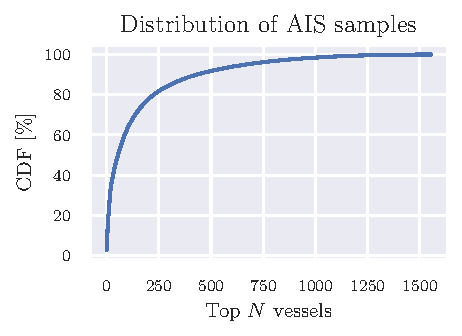
\includegraphics[width=0.5\textwidth]{figures/mmsi_cdf.pdf}
    \caption{Cumulative distribution of \acrshort{ais} messages for the $N$ most frequent vessel's.}
    \label{fig:ais_cdf}
\end{figure}

However, the dataset is currently too large to conveniently work with on a single computer. Two local regions are instead used in this thesis, and they are shown in \cref{fig:ais_data}. The first subset is from a curved section of the Trondheim fjord with a lot of traffic. The subset also includes a ferry crossing, which crosses the traffic lane. The other subset is from deeper into the fjord, from a relatively straight section. The dataset therefore contains both straight-line and curved trajectories, as well as crossing trajectories. 

\begin{figure}
    \centering
    \begin{subfigure}{\textwidth}
        \centering
        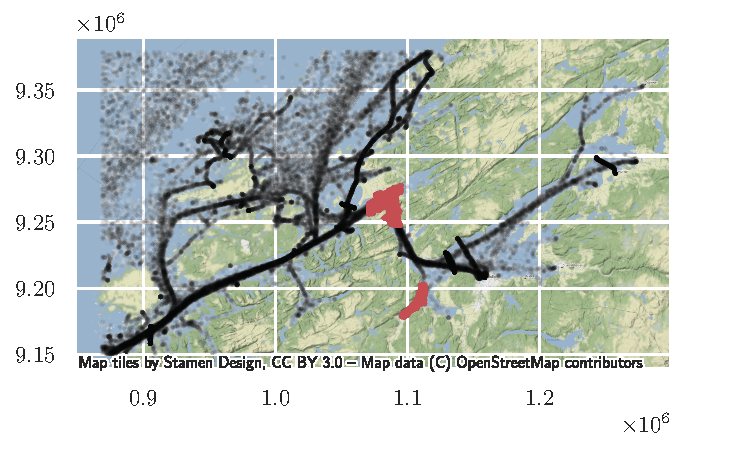
\includegraphics{figures/ais_map.pdf}
        \caption{Full dataset. The blue areas mark the subset that will be used for testing purposes.}
    \end{subfigure}
    \begin{subfigure}{\textwidth}
        \centering
        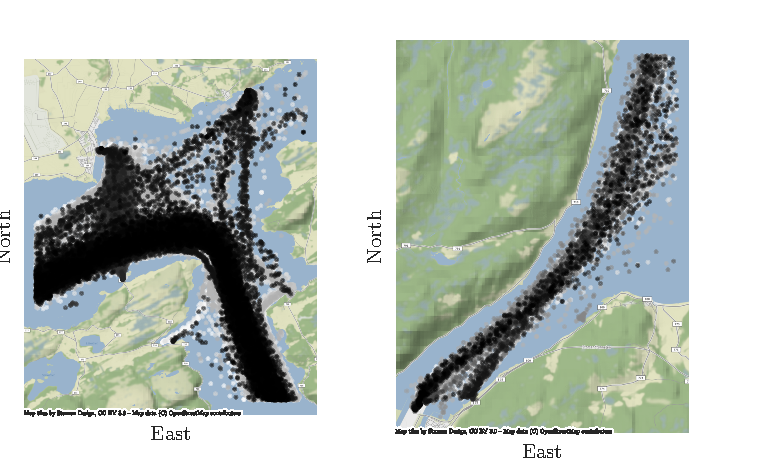
\includegraphics{figures/ais_map_zoom.pdf}
        \caption{Zoomed-in version of the subsets used in this thesis. The blue subset in the left-most map shows the \acrshort{ais} data from three local ferries, which make out more than half of the dataset.}
    \end{subfigure}
    \caption{The available \acrshort{ais} data used in this thesis. }
    \label{fig:ais_data}
\end{figure}

\section{Scenario}
The \acrshort{ais} dataset contains samples from a wide variety of different trajectories, as each trajectory is the result of a vessel's intention, be it reaching a specific destination, commercial fishing, or simply for leisure. As a result, there is a wide range of possible overlapping trajectories that a vessel might follow in any given area. Therefore, this thesis will narrow the problem of long-term prediction down to prediction in specific \textit{scenarios}. A scenario is in this thesis characterized by the vessel's initial position, speed and course, and it is assumed that vessels in a given scenario tend to follow similar trajectories. Though not used in this thesis, it would also be natural to incorporate contextual information such as vessel type, as there is likely quite a lot of variability between the behavior of different types of vessels. 

When predicting the trajectory for a given target vessel, only the subset of \acrshort{ais} messages from similar situations will be used. This simplifying assumption is a critical part of all methods proposed in this thesis. It allows the \acrshort{ais} to be reduced significantly for any given prediction and is what makes the methods computationally feasible. The following requirements must be satisfied for a trajectory to qualify as being in a similar scenario as the target vessel:
\begin{enumerate}
    \item The trajectories' initial position must be close to the target vessel's position $\boldsymbol{x}$. A fixed threshold at $\boldsymbol{x} \pm \Delta \boldsymbol{x}$ is used.
    \item The trajectories' initial \acrshort{cog} must be close to the target vessel's heading $\mathcal{X}$. A fixed threshold at $\mathcal{X} \pm \Delta \mathcal{X}$ is used.
    \item The trajectories' initial \acrshort{sog} must be close to the queried velocity $v$. A fixed threshold at $v \pm \Delta v$ is used.
\end{enumerate}


The notion of only using a small subset of close-by samples from the \acrshort{ais} data is somewhat similar to the SPNS method proposed by \cite{Hexeberg2017AISbasedVT}, though a key distinction is that this thesis selects entire trajectories based on the initial conditions, rather than individual points. 

\subsection{Clustering}
In practical applications, it may be beneficial to use a fixed number of scenarios. For example, clustering-based methods may be used to cluster similar trajectories into a fixed number of scenarios. This approach is not implemented in this thesis but is considered a natural next step.


\section{Preprocessing}
The position (longitude and latitude) is converted from the standard World Geodetic System (WGS84) coordinates into the EUREF89 UTM32 (EPSG-25832) coordinate system \cite{kartverket}.  As a result, the coordinates are converted from spherical coordinates to a 2D euclidian coordinate system, where the first and second axis corresponds to easting and northing, respectively. This coordinate system is one of two official coordinate systems in Norway and yields significantly better projections in this area than other alternatives, such as the Web-Mercator projector frequently used by online maps. Zone 32 is selected as it encompasses the target region.

\subsection{From samples to trajectories}\label{sec:from_ais_to_traj}
Samples with identical \acrshort{mmsi} and less than $15$ minutes between subsequent samples are considered part of the same trajectory. The $15$ minute requirement is added to ensure that samples before and after docking are considered separate trajectories. The length of the trajectories must be between $15$ and $30$ minutes, and the number of samples in each trajectory must be greater than $4$. 
